\documentclass[12pt,a4paper]{article}
\usepackage[margin=2.5cm]{geometry}
\usepackage{amsmath}
\usepackage{amssymb}
\usepackage{graphicx}
\usepackage{booktabs}
\usepackage{multirow}
\usepackage{setspace}
\usepackage{parskip}
\usepackage[hidelinks]{hyperref}
\usepackage{enumitem}
\usepackage{caption}
\usepackage{float}
\usepackage{listings}
\usepackage{xcolor}
\usepackage{lmodern}
\usepackage[T1]{fontenc}

\onehalfspacing

\definecolor{codebg}{rgb}{0.95,0.95,0.95}
\lstset{
  backgroundcolor=\color{codebg},
  basicstyle=\ttfamily\small,
  breaklines=true,
  frame=single,
  language=R
}

\title{\textit{How does Infrastructure Quality Impact GDP?}}
\author{}
\date{}

\begin{document}

\maketitle
\noindent Word Count: 1983

\vspace{1em}

Infrastructure is widely accepted to be a crucial ingredient or a ``pre-requisite'' for economic development (Srinivasu and Rao, 2013). Infrastructure is a broad term, with various types of infrastructure theoretically working as important routes for growth, albeit through different channels. For example, an adequate supply of transport infrastructure, such as roads or ports enables more efficient movement of resources and capital, improving productivity, as well as allowing greater access to global markets to exploit comparative advantages and raise national income. Greater access to electricity or internet may improve productivity within industries, as well as providing an opportunity to grow higher value-added sectors such as manufacturing or information services. The belief in the benefits of infrastructure investment is apparent to this day, with the World Bank spending \$12.8bn on infrastructure development in developing countries in 2023, and Goal 9 of the Sustainable Development Goals specifically referring to infrastructure development.

Despite the claimed benefits and the scale of resources invested, in a review of empirical evidence Timilsina et al. (2020) found there is not a clear consensus on the relationship between infrastructure development and economic growth. Some studies, such as Banerjee et al. (2012) find no significant impact of GDP from proximity to infrastructure, in this case in China, whereas others, for example Sohoo and Dash (2012) find a significant positive impact of infrastructure in India. It is somewhat unsurprising that results differ, as the marginal impact of infrastructure will be heterogeneous, depending on its quality, substitutability with existing infrastructure and local demand.

This tension between theoretical benefits of infrastructure, alongside the scale of resources invested, and the limited economic evidence motivates the research question of this paper: \textbf{``\textit{How does Infrastructure Quality Impact GDP?}''} To answer it, we will use cross sectional data of GDP and Infrastructure Quality, first with a simple OLS model, and then with geographical instrumental variables to mitigate reverse causality.

\section*{Data}

Our key dependent variable is `Infrastructure Score' from the World Bank's Logistics Performance Index (LPI) in 2018, measured by surveying logistics professionals. For the LPI's infrastructure score, respondents are asked to rate the quality of physical infrastructure in their countries of expertise on a scale of 1--5. Relying on survey data is imperfect, as it is subject to sampling error, and the number of respondents varies significantly between countries, leading to disparities in associated confidence intervals. However, the LPI Infrastructure scores are thorough in their breadth, with over 160 countries rated by over 850 respondents, and depth, with 6 separate aspects of infrastructure scored.

We will measure economic output through 2018 per capita Gross Domestic Product. As GDP measures the \textit{value} of a country's annual economic activity, cross-country comparisons can be susceptible to differences in relative prices, which do not reflect underlying economic activity that we are interested in. Therefore, we will use \textit{real} GDP so that we are not influenced by divergent levels of inflation and Purchasing Power Parity (PPP) to control for differences in purchasing power.

We are using cross-sectional data for our variables, rather than panel data, as we will utilise time-invariant geographical instruments, which would not work in a dynamic model.

\section*{Analysis}

\begin{figure}[H]
  \centering
  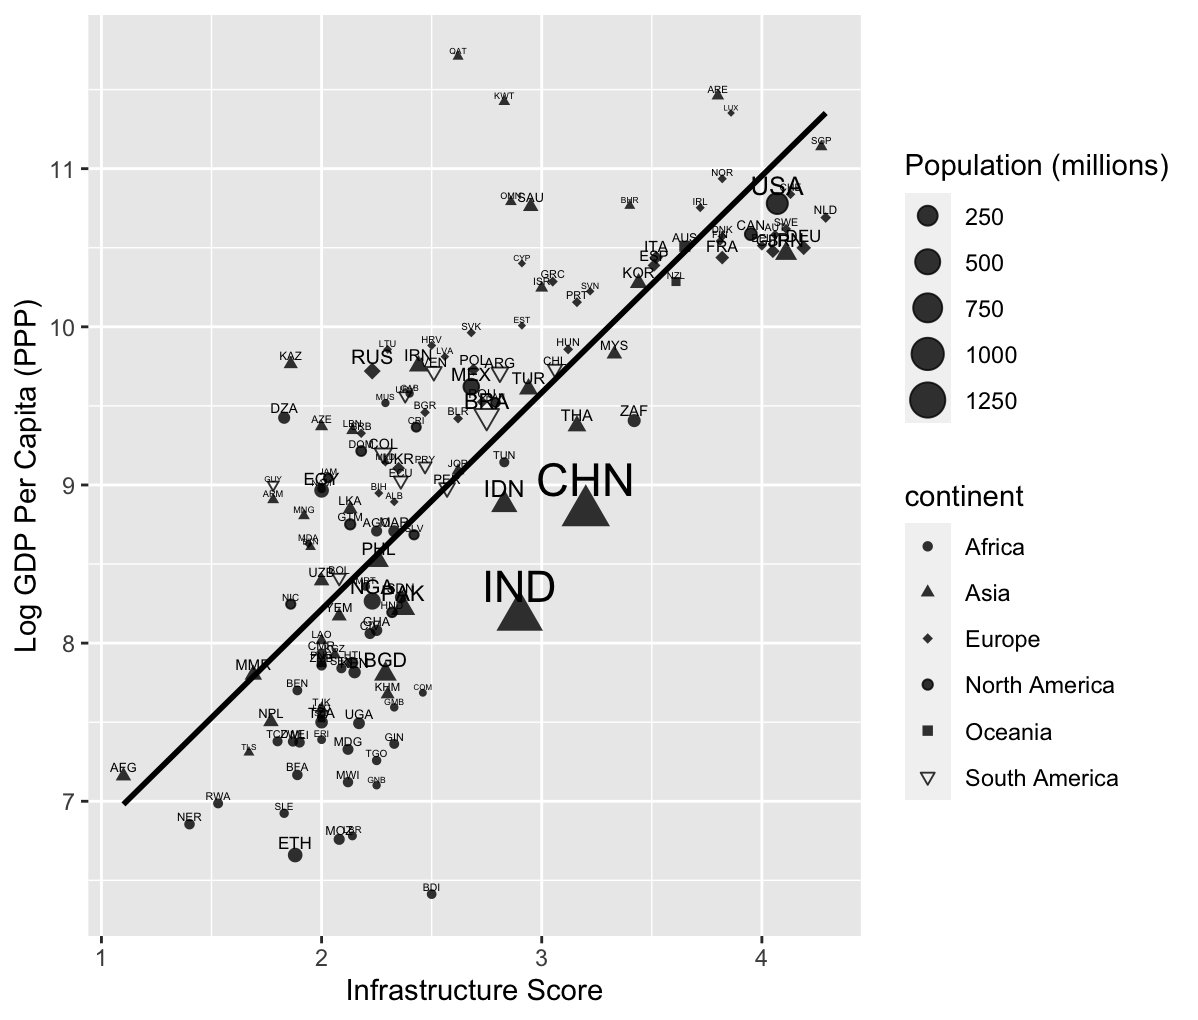
\includegraphics[width=0.9\textwidth]{Rplotshapes.png}
  \caption{Infrastructure Score and Log GDP Per Capita (PPP) in 2018}
  \label{fig:scatter}
\end{figure}

Figure \ref{fig:scatter} shows the strong positive relationship between log GDP per capita (PPP) and infrastructure score. Observations vary in shape according to their continent, and the size of the shape varies depending on the population. The regression line in Figure \ref{fig:scatter} is specified in equation (1):

\begin{equation}
  \log y_i = \beta_0 + \beta_1 \mathit{infra}_i + \varepsilon_i
\end{equation}

Where $\log y_i$ is our dependent variable, log of GDP in country $i$, and $\mathit{infra}_i$ is country $i$'s infrastructure score. The OLS results for the estimation are in column 1 of Table \ref{fig:regtable}, where the coefficient for $\beta_1$ shows that increasing infrastructure score by 1 is associated with a 134\% increase in GDP per capita. Infrastructure score captures a notably large 59\% of the variation in GDP. However, there is strong reason to believe that our variable is endogenous, where our independent variable, $\mathit{infra}_i$ is correlated with the error term $\varepsilon$, which means our estimate of $\beta_1$ is biased.

One likely source for endogeneity here is omitted variable bias. Building and operating high quality infrastructure, especially for complex projects such as ports and airports, requires both educated and healthy workers. Furthermore, stronger legal systems discourage syphoning resources and encourage private investment in infrastructure. Therefore, these variables are likely correlated with both infrastructure development, as well as GDP, and are contained in the error term ($\varepsilon$) in equation (1). Consequently, our estimate of $\beta_1$ will also capture these effects. To mitigate this, in our second regression, shown in equation (2) we will control for:

\begin{enumerate}[label=(\roman*)]
  \item Education: Mean years of schooling in 2018, $\mathit{educ\_level}$ in equation (2), from the UNDP Human Development Report (2022).
  \item Rule of Law: A rule of law index, $\mathit{law\_quality}$ in equation (2) produced by the University of Gothenburg in 2018, measuring judicial independence, transparency, and accessibility, alongside corruption. The index ranges from 0 to 1 (most rule based).
  \item Health: Life expectancy at birth, $\mathit{life\_exp}$ in equation (2), measured by the UNN WPP, in 2018.
\end{enumerate}

These sources were chosen for their reliability, and for including the largest selection of countries possible.

\begin{equation}
  \log y_i = \alpha_0 + \alpha_1 \mathit{infra}_i + \alpha_2 \mathit{educ\_level}_i + \alpha_3 \mathit{law\_quality}_i + \alpha_4 \mathit{life\_exp}_i + u_i
\end{equation}

We use OLS again to estimate Equation (2) in column 2 of Table \ref{fig:regtable}. These 4 variables explain a remarkable 86\% of the variation in GDP. While infrastructure score remains statistically significant in the second regression, the marginal impact of an extra point, $\alpha_1$, is a much more modest 33\% increase in GDP per capita. Education quality and life expectancy are also statistically significant predictors of GDP, although the rule of law variable is not statistically significant. However, we still cannot conclude with any confidence that we have captured any causal estimate of infrastructure quality on GDP. Firstly, we are unlikely to have captured all important omitted variables. Trade openness and peaceful relations with neighbouring countries are also likely to be correlated with both infrastructure quality and GDP. However, both variables are difficult to measure, and available sources tend to only include a small subsection of countries.

Another source of endogeneity is reverse causality. Here the bias arises from the fact that countries with higher GDP per capita are likely to have greater resources in which to invest in infrastructure. Therefore, it is likely we are not only capturing the impact of infrastructure quality on GDP, but also the impact of GDP on infrastructure quality. Reverse causality is a recurring problem in the literature of economic output and infrastructure, especially where OLS is used (Timilsina et al., 2020). It should also be noted that our control variables in equation (2) are also all susceptible to reverse causality, as richer countries will have greater resources will be able to invest in increasing the number of years of education, life expectancy and a more effective legal system.

To mitigate this we will use three geographic instrumental variables, which will be used to predict infrastructure score. GDP per capita will then be regressed on our fitted values of infrastructure. As these instrumental variables are geographic, they cannot be caused by GDP, addressing endogeneity from reverse causality. These geographic instruments were chosen because they provide us with the highest possible F stat from the instruments examined (including terrain ruggedness, desert and island variables).

\begin{enumerate}[label=(\roman*)]
  \item $\mathit{coastline}$ is a measure of kilometres of coastline, as recorded in the CIA World Fact Book (n.d.). This captures the fact that countries with large coastlines have more opportunities to trade, and can experience higher returns to infrastructure by accessing global markets more easily.
  \item $\mathit{rainforest\_dummy}$ uses rainfall data from the WorldBank, and classifies those with rainfall of at least 2,000 mm per year as rainforests (NASA, n.d.). Heavily forested areas make construction more difficult and result in fewer agglomerations, decreasing returns to infrastructure.
  \item $\mathit{coastline\_dummy}$ is a dummy variable of whether a country has a coastline. Much like with our coastline variable, countries with a coastline can access global markets, incentivising infrastructure investment.
\end{enumerate}

The first stage of our instrumental variable (IV) regression is shown in equation (3):

\begin{equation}
  \mathit{infra}_i = \gamma_0 + \gamma_1 \mathit{coastline}_i + \gamma_2 \mathit{rainforest\_dummy}_i + \mathit{coastline\_dummy}_i + \eta_i
\end{equation}

For an instrumental variable to be valid, there are two central considerations. Firstly, the instrument must be a relevant predictor of our endogenous variable, infrastructure score. This is what we test for in the first stage of our 2-stage least squares (2SLS) regression. In column 3 of Table \ref{fig:regtable}, we can see 3 of our instruments are significant at the 1\% level, as is our F-stat of joint significance, implying our instruments are not weak. In fact, the three geographical instruments explain around 19\% of the variation in infrastructure quality.

\begin{equation}
  \log y_i = \delta_0 + \delta_1 \mathit{infra}_i + \delta_2 \mathit{africa\_dummy}_i + \delta_3 \mathit{asia\_dummy}_i + \mu_i
\end{equation}

The second requirement for IV validity is the exclusion criteria, which requires that in our second stage of the 2SLS regression, equation (4), the only way in which our instruments influence our dependent variable is through our predicted variable, $\mathit{infra}_i$. This criteria is much less likely to have been met. Geographic variables of coastline length, rainforest dummy and coastline dummy are likely to also influence other aspects of GDP. For example, Lane and Pretes (2020) find a significant relationship between access to maritime trade, which is heavily influenced by our coastline instruments, and GDP. However, omitted variables such as trade dependence are likely endogenous, and would require further instrumental variables, therefore they are not included in our regression. Secondly, our geographic instruments are predictors of continent, as different continents have different coastline ratios and rainfall levels. Therefore, we may in fact just be predicting continental GDP. To control for continent specific factors, we include Africa and Asia dummy variables in equation (4). In column 4 of Table \ref{fig:regtable}, we have also included the P value for the Sargan overidentification test (as we have three instruments for a single endogenous variable). In the Sargan test, our hypothesis is that all our instruments are valid, as they are not correlated with the error term $\mu$. Our P-value implies we very narrowly fail to reject this at the 5\% level, however, as discussed above, there is likely evidence that the instruments do not fulfil the exclusion restriction.

While not as high as our first specification, column 4 in Table \ref{fig:regtable} suggests the returns to increasing infrastructure score are incredibly high, with an increase of 1 associated with a 112\% increase in GDP per capita. Our continent dummies are also statistically significant. However, because we cannot assume we have fulfilled the exclusion requirement, again we cannot claim that this figure is representative of the causal relationship between infrastructure and growth.

\begin{table}[H]
\centering
\caption{Full Regression Table for Infrastructure and GDP}
\label{fig:regtable}
\begin{tabular}{lcccc}
\toprule
 & \multicolumn{4}{c}{\textit{Dependent variable:}} \\
\cmidrule(lr){2-5}
 & \multicolumn{2}{c}{log\_gdp} & infrastructure\_score & log\_gdp \\
 & (1) & (2) & (3) & (4) \\
\midrule
infrastructure\_score & 1.344$^{***}$ & 0.329$^{***}$ & & \\
 & (0.095) & (0.089) & & \\[4pt]
educ\_level & & 0.126$^{***}$ & & \\
 & & (0.018) & & \\[4pt]
law\_quality & & $-$0.038 & & \\
 & & (0.166) & & \\[4pt]
life\_exp & & 0.071$^{***}$ & & \\
 & & (0.008) & & \\[4pt]
coastline & & & 0.00001$^{***}$ & \\
 & & & (0.00000) & \\[4pt]
rainforest\_dummy & & & $-$0.522$^{***}$ & \\
 & & & (0.147) & \\[4pt]
coastline\_dummy & & & 0.393$^{***}$ & \\
 & & & (0.121) & \\[4pt]
infra\_instrument & & & & 1.116$^{***}$ \\
 & & & & (0.238) \\[4pt]
africa\_dummy & & & & $-$1.785$^{***}$ \\
 & & & & (0.164) \\[4pt]
asia\_dummy & & & & $-$0.495$^{***}$ \\
 & & & & (0.162) \\[4pt]
Constant & 5.779$^{***}$ & 2.285$^{***}$ & 2.492$^{***}$ & 7.021$^{***}$ \\
 & (0.269) & (0.455) & (0.103) & (0.676) \\
\midrule
Model Type & OLS & OLS & IV & 2SLS \\
Sargan Overid.\ P-Value & & & & 0.0508 \\
Observations & 142 & 142 & 142 & 142 \\
R$^2$ & 0.589 & 0.861 & 0.187 & 0.532 \\
Adjusted R$^2$ & 0.587 & 0.857 & 0.169 & 0.522 \\
Residual Std.\ Error & 0.741 & 0.436 & 0.601 & 0.797 \\
F Statistic & 201.039$^{***}$ & 211.964$^{***}$ & 10.552$^{***}$ & 52.263$^{***}$ \\
\bottomrule
\multicolumn{5}{l}{\footnotesize $^*$p$<$0.1; $^{**}$p$<$0.05; $^{***}$p$<$0.01} \\
\end{tabular}
\end{table}

\section*{Limitations and Evaluation}

In this paper, we have deployed both OLS and 2SLS methods to estimate the impact of infrastructure on output. Despite the endogeneity concerns, as all our coefficients for this relationship were large, positive, and strongly statistically significant, this paper aligns with much of the literature and economic theory, that high quality infrastructure likely positively impacts GDP. However, there is much more difficulty in claiming any findings when measuring the extent of the relationship. Indeed, this is not a unique problem with infrastructure, almost all explanatory variables of development will have elements of reverse causality, as many of the outcomes that are associated with greater wealth (health, education, institutions etc.) impose a cost on the state. Instrumental variables are one method to deal with this, but as shown here, and in many other areas of economic literature it is very difficult to find an instrument that satisfies both the exclusion and relevance criteria.

\section*{Bibliography}

\subsection*{(i) Data}

\begin{itemize}[leftmargin=2em]
  \item \textit{Connecting to compete 2018: LPI Trade Logistics in the global economy}. (2018) World Bank. Available at: \url{https://openknowledge.worldbank.org/handle/10986/29971}
  \item \textit{Average precipitation in depth (mm per year)} (2024) World Bank Open Data. Available at: \url{https://data.worldbank.org/indicator/AG.LND.PRCP.MM}
  \item \textit{Land area (sq.\ km)} (2024) World Bank Open Data. Available at: \url{https://data.worldbank.org/indicator/AG.LND.TOTL.K2}
  \item \textit{Central Intelligence Agency World Fact Book} (No date). Available at: \url{https://www.cia.gov/the-world-factbook/field/coastline/}
  \item \textit{Human development report 2021--22}. (2022) Human Development Reports. Available at: \url{https://hdr.undp.org/content/human-development-report-2021-22}
  \item \textit{Rule of law index} (no date) Our World in Data. Available at: \url{https://ourworldindata.org/grapher/rule-of-law-index?time=2018}
  \item \textit{Life expectancy} (no date) Our World in Data. Available at: \url{https://ourworldindata.org/grapher/life-expectancy?tab=map&time=2018}
\end{itemize}

\subsection*{(ii) Literature and Other Sources}

\begin{itemize}[leftmargin=2em]
  \item \textit{Rainforest: Mission: Biomes} (no date) NASA. Available at: \url{https://earthobservatory.nasa.gov/biome/biorainforest.php}
  \item Srinivasa and Rao (2016) \textit{Infrastructure Development and economic growth: Prospects and perspective}, Academia.edu. Available at: \url{https://www.academia.edu/24400230/Infrastructure_Development_and_Economic_growth_Prospects_and_Perspective}
  \item Timilsina, Govinda \& Hochman, Gal \& Song, Ze. (2020). \textit{Infrastructure, Economic Growth, and Poverty: A Review}. 10.1596/1813-9450-9258.
  \item Banerjee, Duflo \& Qian (2012). \textit{On the Road: Access to Transportation Infrastructure and Economic Growth in China}. NBER Working Papers 17897, National Bureau of Economic Research, Inc. \url{https://ideas.repec.org/p/nbr/nberwo/17897.html}
  \item Sahoo, P., \& Dash, R. K. (2012). Economic growth in South Asia: Role of infrastructure. \textit{The Journal of International Trade \& Economic Development}, 21(2), 217--252.
  \item Lane, Jesse \& Pretes, Michael. (2020). Maritime dependency and economic prosperity: Why access to oceanic trade matters. \textit{Marine Policy}. 121. 104180. 10.1016/j.marpol.2020.104180.
\end{itemize}

\subsection*{AI Prompts}

I used ChatGPT for Figure \ref{fig:scatter}:\\
Prompt: \textit{How can I show GGPlot groups as shapes rather than colours.}\\
This instructed me to use the specified shapes, as seen in Appendix A.

\appendix

\section{Full Code in R}

\lstinputlisting[language=R]{analysis.r}

\end{document}
